\documentclass[a4paper]{article}

% formatting
\usepackage[utf8]{inputenc} % allow utf-8 input
\usepackage[T1]{fontenc} % use 8-bit T1 fonts  (allows for direct use of ö,ü,etc.)

% math typesetting
\usepackage{amsmath}
\usepackage{amssymb}
\usepackage{amsfonts}

% maths definitions, theorems, etc.
\usepackage{amsthm}

% color
\usepackage{color}
\usepackage{xcolor}

% layout
\usepackage{layout}
\usepackage{lipsum}

% cross-referencing and hyperlinks
\usepackage{hyperref}
\usepackage{url}
\usepackage{doi}

% figures
\usepackage{graphicx}
\usepackage{subfig}
\usepackage{wrapfig}

% tables
\usepackage{booktabs}
\usepackage{multirow}
\usepackage{caption} 
\usepackage{float}

% enumeration
\usepackage{enumitem}

% embedding pages
\usepackage{pdfpages}

% multi-line comments
\usepackage{comment}

% landscape orientation
\usepackage{rotating}
\usepackage{pdflscape}

% Gantt charts
\usepackage{pgfgantt}

% footnotes
\usepackage{footnote}

% code
\usepackage{listings}

% matrices and tables
\usepackage{nicematrix}
\usepackage{varwidth}
% \usepackage{tabularx} do not load package tabularx, instead use package nicematrix

% document structure
\setcounter{secnumdepth}{5} % enable numbered sub-sub-sections etc.

% custom header size
\usepackage{titlesec}

% customized references (make "Figure 1" a link, not just "1")
\usepackage[capitalise, nameinlink]{cleveref}

% customized frames around text etc.
\usepackage{mdframed}

% tikz
\usepackage{tikz}

% calligraphy
\usepackage{calligra}

% chemical formulas
\usepackage{chemformula}
% column layout
\usepackage{multicol}
\setlength{\columnsep}{0.75cm}

% paragraphs
\usepackage[skip=0.5\baselineskip]{parskip}

% geometry
\usepackage[
    margin = 3cm,
    top = 3cm,
    bottom = 3cm
]{geometry}

% header size
\usepackage{titlesec}
\titleformat*{\section}{\large\bfseries}
\titleformat*{\subsection}{\normalsize\bfseries}
\titleformat*{\subsubsection}{\normalsize\bfseries}
\titleformat*{\paragraph}{\normalsize\bfseries}
\titleformat*{\subparagraph}{\normalsize\bfseries}

% custom headers
\usepackage{fancyhdr}
\pagestyle{fancy}
\fancyhead{}
\fancyfoot{}
\renewcommand{\headrulewidth}{0.4pt} % Keep header line
\setlength{\headheight}{15pt}
\setlength{\headsep}{10pt}
\renewcommand{\sectionmark}[1]{}
\renewcommand{\subsectionmark}[1]{}

\usepackage[
    backend=biber,
    style=ieee
]{biblatex}
\addbibresource{references.bib}
% show DOI URL (https://doi.org/XXX.XXXXX.XXXX), instead of publisher URL (https://springer.com/XXXX)
% cf. https://tex.stackexchange.com/a/616241
\DeclareSourcemap{
  \maps[datatype = bibtex]{
    \map{
      \step[notfield = keywords, final]
      \step[fieldsource = doi, final]
      \step[fieldset = url, null]
    }
    \map{
      \step[fieldsource = keywords, notmatch = \regexp{\bprimary\b}, final]
      \step[fieldsource = doi, final]
      \step[fieldset = url, null]
    }
  }
}
\AtEveryBibitem{
    \clearfield{urlyear}
    \clearfield{urlmonth}
}

\usepackage{tikz}

% https://tex.stackexchange.com/a/294990
\newcommand{\ExternalLink}{
    \tikz[x=1.2ex, y=1.2ex, baseline=-0.05ex]{
        \begin{scope}[x=1ex, y=1ex]
            \clip (-0.1,-0.1) 
                --++ (-0, 1.2) 
                --++ (0.6, 0) 
                --++ (0, -0.6) 
                --++ (0.6, 0) 
                --++ (0, -1);
            \path[draw, 
                line width = 0.5, 
                rounded corners=0.5] 
                (0,0) rectangle (1,1);
        \end{scope}
        \path[draw, line width = 0.5] (0.5, 0.5) 
            -- (1, 1);
        \path[draw, line width = 0.5] (0.6, 1) 
            -- (1, 1) -- (1, 0.6);
        }
    }

\renewcommand{\contentsname}{\centering Contents} % https://tex.stackexchange.com/a/308207
\usepackage[titles, subfigure]{tocloft} % https://tex.stackexchange.com/a/336618
\renewcommand{\cftsecleader}{\cftdotfill{\cftdotsep}} % https://tex.stackexchange.com/a/271942

%%%%%%%%%%%%%%%%%%%%%%%%%%%%%%%%%%%%%%%%%%%%%%%%%%%%%%%%%%%%%%%%%%%%%

% document metadata
\title{Proposal for a Summer Academy \protect\\ on Biophilic Design in Architecture}
\author{Michael P. Weinold$^1$, Philippe Schultheiss$^1$, Mark C. Ballandies$^2$}
\date{
    $^1$Schweizerische Studienstiftung \\
    $^2$Stiftung der Deutschen Wirtschaft \\[3mm]
    October 2023
}

%%%%%%%%%%%%%%%%%%%%%%%%%%%%%%%%%%%%%%%%%%%%%%%%%%%%%%%%%%%%%%%%%%%%%

\begin{document}

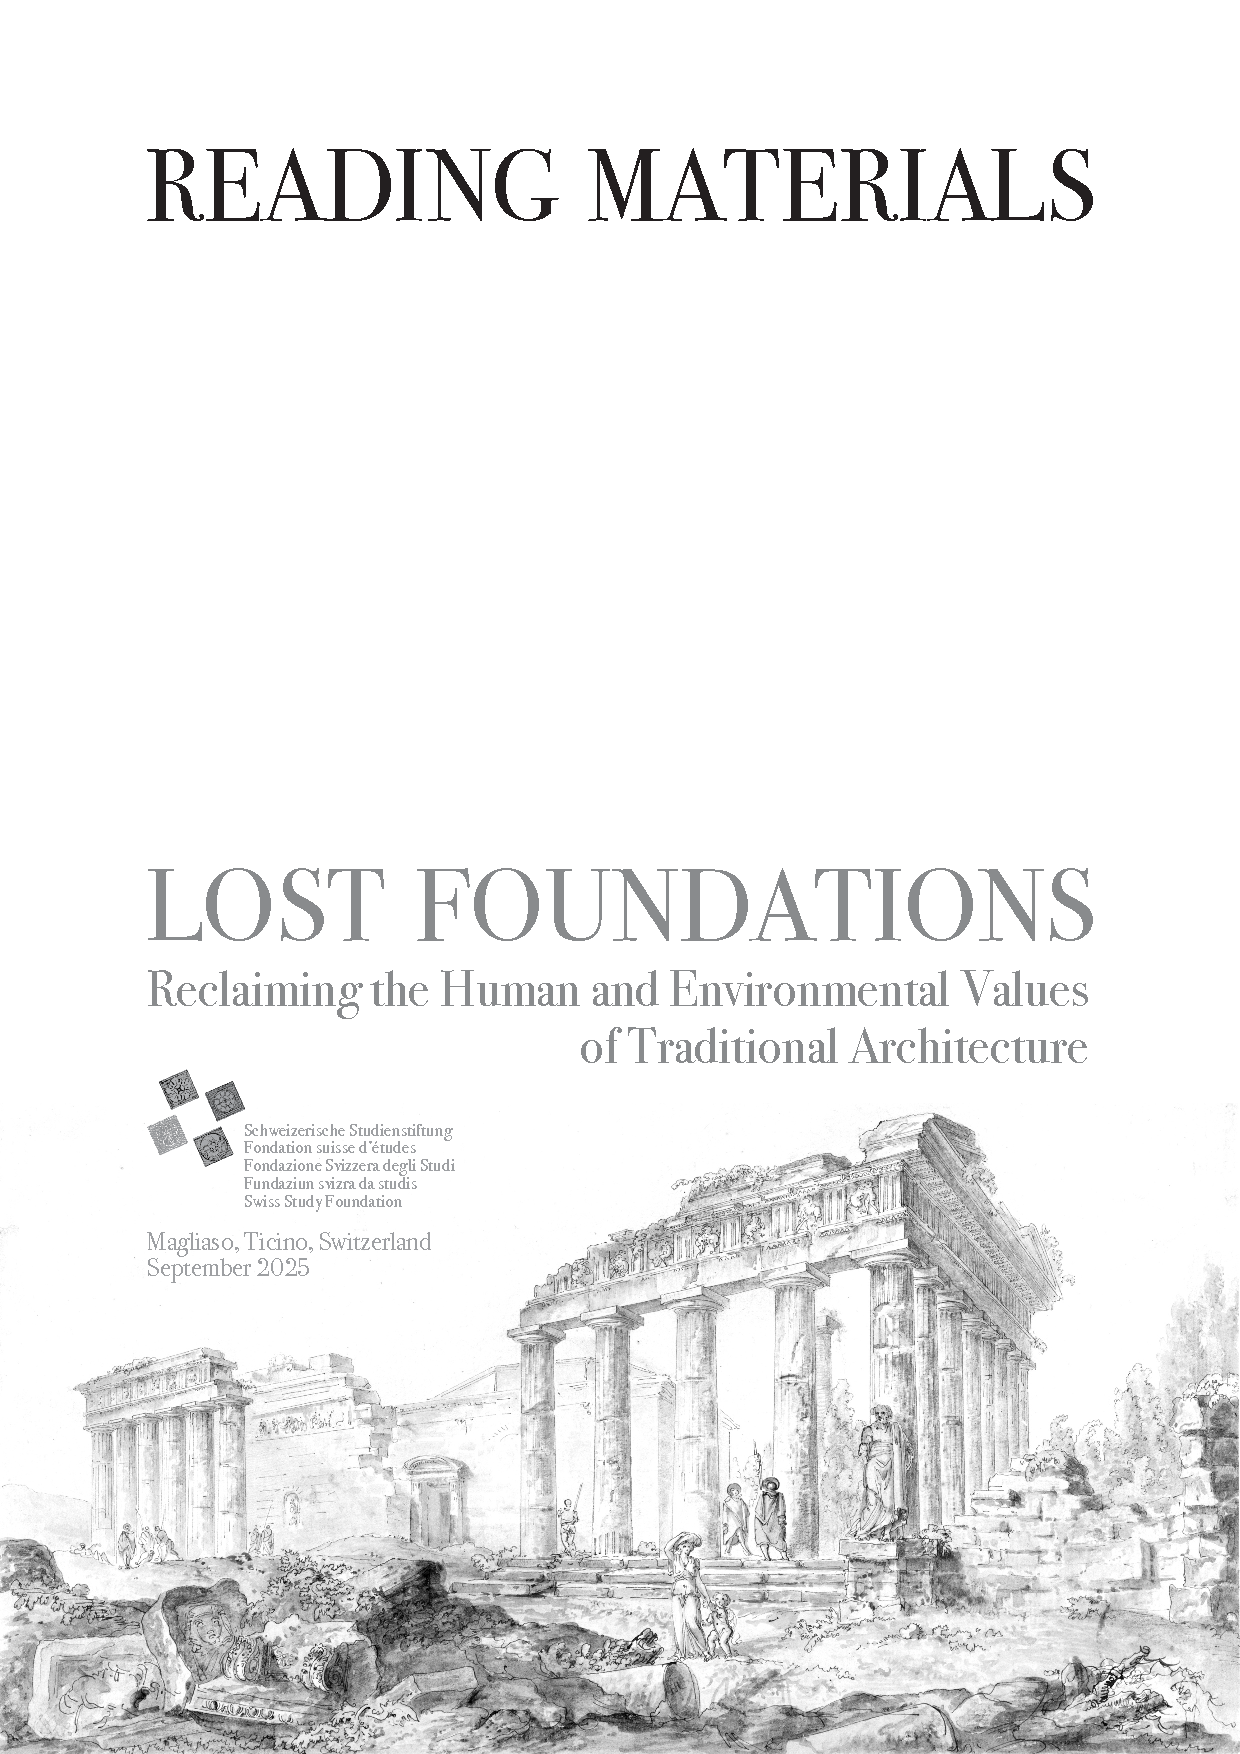
\includepdf[pages=1-2]{figures/cover.pdf}

\clearpage

\section*{\centering Introduction}

In the womb the human embryo passes through all the development stages of the animal kingdom. At the moment of birth, human sensations are equal to those of a newborn dog. His childhood passes through all the transformations which correspond to the history of mankind. At the age of two, he sees like a Papuan, at four, like a Teuton, at six like Socrates, at eight like Voltaire. When he is eight years old, he becomes aware of violet, the colour which the eighteenth century had discovered, because before that the violet was blue and the purple snail red. Today the physicist points to colours in the sun’s spectrum which already bear a name, whose recognition, however, is reserved for the coming generation.

The child is amoral. To us the Papuan is also amoral. The Papuan slaughters his enemies and devours them. He is no criminal. If, however, the modern man slaughters and devours somebody, he is a criminal or a degenerate. The Papuan tattoos his skin, his boat, his oar, in short, everything that is within his reach. He is no criminal. The modern man who tattoos himself is a criminal or a degenerate. There are prisons where eighty percent of the inmates bear tattoos. Those who are tattooed but are not imprisoned are latent criminals or degenerate aristocrats. if a tattooed person dies at liberty, it is only that he died a few years before he committed a murder.

% https://tex.stackexchange.com/a/244104/
\begin{tikzpicture}[remember picture,overlay]
    \node[xshift=-1.2cm,yshift=+3.2cm] at (current page.south east) {
\includegraphics[height=8cm]{./figures/dandelion.jpg}};
\end{tikzpicture}
\begin{tikzpicture}[remember picture, overlay]
    \node[xshift=-10.3cm, yshift=+0.75cm, font=\small] at (current page.south east) {\textit{two dandelions of the genus Taraxacum, most often associated with the archetype of flowers springing from concrete}};
\end{tikzpicture}

\section*{\centering Administrative Information}

All supporting materials of the Summer Academy are available in a Zenodo repository under a Creative Commons license at \href{https://doi.org/10.5281/zenodo.14575784}{\texttt{doi:10.5281/zenodo.14575784}}. You may reach the authors at:

\begin{NiceTabularX}{\textwidth}{llX}
\textit{Author} & \textit{Email} & \textit{Phone} \\
\hline
Michael P. Weinold & \texttt{michael@weinold.ch} & \texttt{+41 75 500 70 70} \\
Philippe Schultheiss & \texttt{phschultheiss@protonmail.ch} & \texttt{+41 79 768 53 15} \\
Mark C. Ballandies & \texttt{bcmark@protonmail.com} & \texttt{+41 78 899 87 85}
\end{NiceTabularX}

\begin{figure}[h]
  \centering
  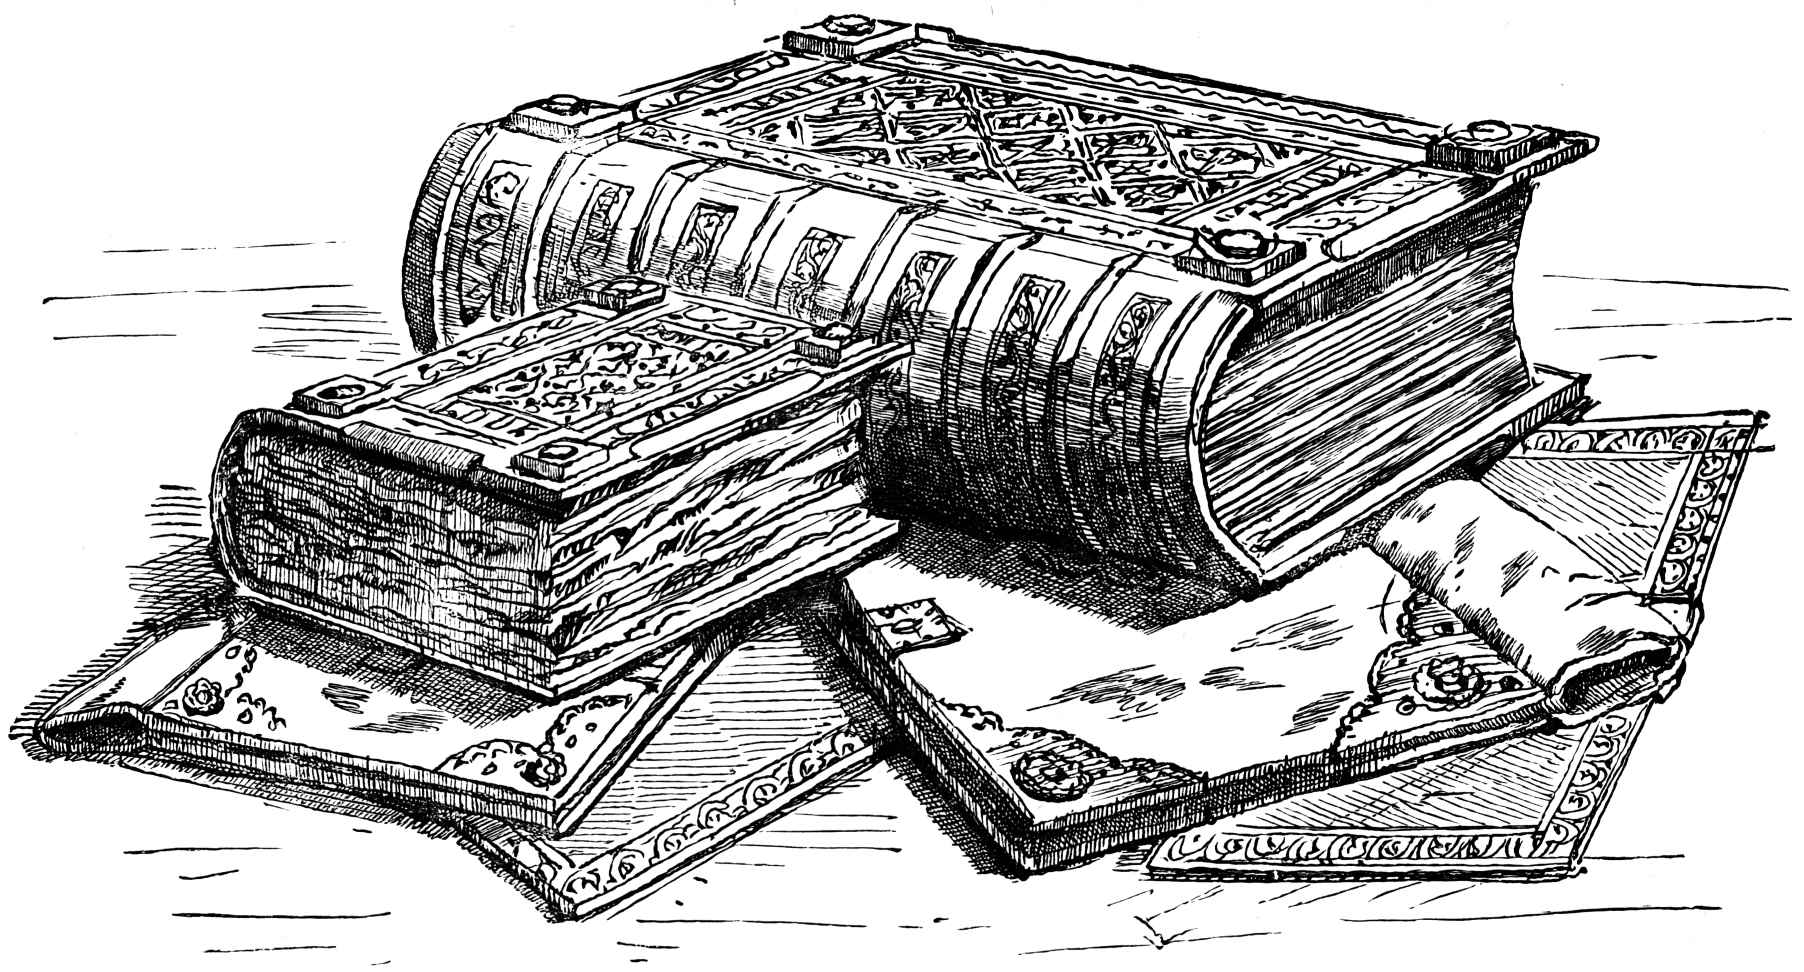
\includegraphics[width=0.4\textwidth]{./figures/books.jpg}
\end{figure}

\tableofcontents

\clearpage
\section{Architecture History}

\begin{mdframed}[linewidth=1pt, roundcorner=5pt, innerleftmargin=10pt, innerrightmargin=10pt, innertopmargin=10pt, innerbottommargin=10pt, linecolor=black, backgroundcolor=white, userdefinedwidth=\textwidth]
    To better understand the intellectual dimension of the early modern movement against traditional architecture, it is essential to examine the writings and theories of its key figures, particularly those who challenged the prevailing aesthetic norms. Perhaps most well known among those is \textit{Ornament und Verbrechen} \cite{loos_ornament_1908} (en: "Ornament and Crime"). This short essay was originally delivered as a lecture to the Vienna-based \textit{Akademischer Verband fur Literatur und Musik} on 21 January 1910 by Austrian architect Adolf Loos. His most well-known work in Vienna, the mixed-use \textit{Looshaus}, stands in stark contrast to the famous \textit{Secessionsgebäude} completed only some 20 years earlier. With it, Loos pioneered the use of reinforced concrete in an otherwise brick-built city. A controversial design, even in its own time, it famously omitted the lavish ornamental decorations otherwise used on both representative and residential buildings of the city. \cref{fig:caricature_loos} shows a contemporary caricature speculating on Loos' inspiration for the design of the main façade.

    \centering % Center the image and caption within the mdframed box
    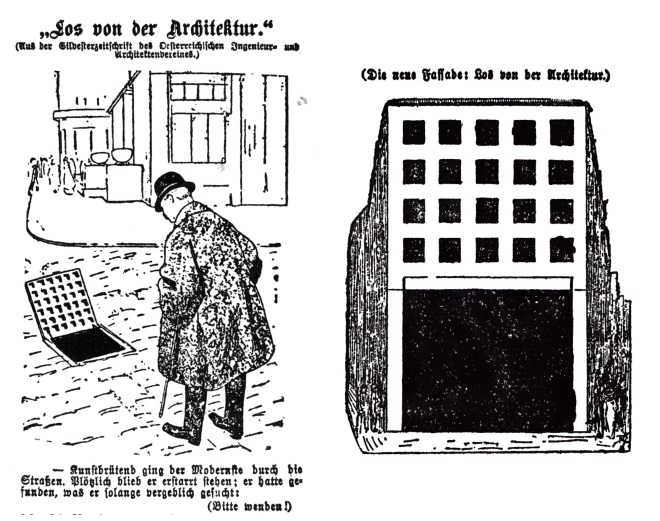
\includegraphics[width=0.7\linewidth]{./figures/caricature_loos.jpg} % Adjusted to \linewidth for consistency within the box
    \captionof{figure}{\textit{"Kunstbrütend ging der Modernste durch die Stassen. Plötzlich blieb er erstarrt stehen. Er hatte gefunden was er solange vergeblich gesucht: Die neue Fassade: Los von der Architektur!"} (en: "Artfully brooding, the most modern one walked through the streets. Suddenly, he stopped, frozen. He had found what he had long sought in vain: The new facade: Free from architecture!"). Contemporary caricature of Adolf Loos, published 1911 in the Viennese newspaper \textit{Illustrirtes Wiener Extrablatt}.}
    \label{fig:caricature_loos}
\end{mdframed}

\subsection{Ornament and Crime (Adolf Loos, 1910)}

In the womb the human embryo passes through all the development stages of the animal kingdom. At the moment of birth, human sensations are equal to those of a newborn dog. His childhood passes through all the transformations which correspond to the history of mankind. At the age of two, he sees like a Papuan, at four, like a Teuton, at six like Socrates, at eight like Voltaire. When he is eight years old, he becomes aware of violet, the colour which the eighteenth century had discovered, because before that the violet was blue and the purple snail red. Today the physicist points to colours in the sun’s spectrum which already bear a name, whose recognition, however, is reserved for the coming generation.

The child is amoral. To us the Papuan is also amoral. The Papuan slaughters his enemies and devours them. He is no criminal. If, however, the modern man slaughters and devours somebody, he is a criminal or a degenerate. The Papuan tattoos his skin, his boat, his oar, in short, everything that is within his reach. He is no criminal. The modern man who tattoos himself is a criminal or a degenerate. There are prisons where eighty percent of the inmates bear tattoos. Those who are tattooed but are not imprisoned are latent criminals or degenerate aristocrats. if a tattooed person dies at liberty, it is only that he died a few years before he committed a murder.

The urge to ornament one’s face, and everything in one’s reach, is the origin of fine art. It is the babble of painting. All art is erotic.

The first ornament that came into being, the cross, had an erotic origin. The first work of art, the first artistic action of the first artist daubing on the wall, was in order to rid himself of his natural excesses. A horizontal line: the reclining woman. A vertical line: the man who penetrates her. The man who created it felt the same urge as Beethoven, he experienced the same joy that Beethoven felt when he created the Ninth Symphony.
But the man of our time who daubs the walls with erotic symbols to satisfy an inner urge is a criminal or a degenerate. It is obvious that his urge overcomes man: such symptoms of degeneration most forcefully express themselves in public conveniences. One can measure the culture of a country by the degree to which its lavatory walls are daubed. With children it is a natural phenomenon: their first artistic expression is to scrawl on the walls erotic symbols. But what is natural to the Papuan and the child is a symptom of degeneration in the modern man. I have made the following observation and have announced it to the world: The evolution of culture is synonymous with the removal of ornament from objects of daily use. I had thought to introduce a new joy into the world: but it has not thanked me for it. Instead the idea was greeted with sadness and despondency. What cast the gloom was the thought that ornament could no longer be produced. What Are we alone, the people of the nineteenth century, are we no longer capable of doing what any Negro can do, or what people have been able to do before us?
Those objects without ornament, which mankind had created In earlier centuries, had been carelessly discarded and destroyed. We possess no carpenter’s benches of the Carolingian period: instead any rubbish which had even the smallest ornament was collected, cleaned and displayed in ostentatious palaces that were built for them, people walked about sadly amongst the display cabinets. Every period had its style: why was it that our period was the only one to be denied a style? By “style” was meant ornament. I said, “Weep not. Behold! What makes our period as important is that it is incapable of producing new ornament. We have outgrown ornament, we have struggled through to a state without ornament. Behold, the time is at hand, fulfilment awaits us. Soon the streets of the cities will glow like white wand Like Zion, the Holy City, the capital of heaven. It is then that fulfilment will have come.”

But there are still hobgoblins who will not allow it to happen. Humanity is still to groan under the slavery of ornament. Man had progressed enough for ornament to no longer produce erotic sensations in him, unlike the Papuans, a tattooed face did not increase the aesthetic value, but reduced it. Man had progressed far enough to find pleasure in purchasing a plain cigarette case, even if it cost the same as one that was ornamented. They were happy with their clothes and they were glad that they did not have to walk about in red velvet trousers with gold braids like monkeys at a fun fair. And I said: “Behold, Goethe’s death chamber is more magnificent than all the pomp of the Renaissance, and a plain piece of furniture is more beautiful than all the inlaid and carved museum pieces. Goethe’s language is more beautiful than all the ornaments of the shepherds of the Pegnitz.”

This was heard by the hobgoblins with displeasure. The state, whose duty it is to impede people in their cultural development, took over the question of development and re-adoption of ornament and made it its own. Woe betide the state, whose revolutions are brought about by its privy councillors!
Soon one was to see a buffet introduced into the Viennese Museum of Applied Arts, which was called “the prosper°us fish shoal,” them was even a cupboard, which was given the trade name “the cursed princess” or something similar, which referred to the ornament with which this unfortunate piece of furniture was covered. The Austrian state takes its task an seriously that it ensures that outdated footwear will not disappear from within the boundaries of the Austro-Hungarian Empire. The state forces every cultivated twenty-year-old man to wear outdated footwear for three years (after all, every state proceeds on the assumption that a poorly developed population is more easily governed). Well, the epidemic of ornament is recognised by the state and is subsidised with government money. I, however, consider that to be a regressive. I will not subscribe to the argument that ornament increases the pleasure of a life of a cultivated person, or the argument which covers itself with the words: “But if the ornament is beautiful!…” To me, and to all the cultivated people, ornament does not increase the pleasures of life. If I want to eat a piece of gingerbread I will choose one that is completely plain and not a piece which represents a baby in arms of a horserider, a piece which is covered over and over again with decoration. The man of the fifteenth century would not understand me. But modern people will. The supporter of ornament believes that the urge for simplicity is equivalent to self-denial. No, time professor from the College of Applied Arts, I am not denying myself! To me, it tastes better this way. The dishes of the past centuries which used decoration to make the peacocks, pheasants and lobsters appear more appetising produce the opposite effect on me. I look on such a culinary display with horror when I think of having to eat these stuffed animal corpses. I eat roast beef.

The immense damage and devastation which the revival of ornament has caused to aesthetic development could easily be overcome because nobody, not even the power of the state, can stop the evolution of humanity! It represents a crime against the national economy, and, as a result of it, human labour, money and material are mined. Time cannot compensate for this kind of damage.

The rate of cultural development is held back by those that cannot cope with the present. I live in the year 1908, but my neighbour lives approximately in the year Iwo, and one over there lives in the year 1880. It is a misfortune for any government, if the culture of its people is dominated by the past. The farmer from gals lives in the twelfth century, and on the occasion of the Jubilee Procession, tribes walked past which even during the period of mass migration were thought to be backward. Happy is the country which does not have such backward-looking inhabitants. Happy is America! Even here we have people in the cities who are survivors from the eighteenth century, and who are appalled by a painting with violent shadows, bemuse they cannot understand why the artist has used violet. To them, the pheasant which the cook has spent days preparing tastes better, and the cigarette case with Renaissance ornaments is more pleasing. And what Is happening in the countryside? Clothes and household utensils belong to previous centuries. The farmer is no Christian, he is still a heathen.

Those who measure everything by the past impede the cultural development of nations and of humanity itself. Ornament is not merely produced by criminals, it commits a crime itself by damaging national economy and therefore its cultural development. Two people living side by side who have the same needs, the same demands on life, and the same income, but belong to different cultures, perceive the national economy differently. The result is that the man of the twentieth century becomes richer and the man of the eighteenth century becomes poorer. I assume that both their lifestyles reflect their different attitudes. The man of the twentieth century can satisfy his needs with a much smaller capital and can, therefore, set aside savings. The vegetable which is appetising to him is simply boiled in water and has butter spread over it. To the other man it will only taste good if honey and nuts are added to it and it has been cooked by someone for hours. Decorated plates are expensive, while white crockery, which is pleasing to the modern individual, is cheap. Whilst one person saves money, the other becomes insolvent. This is what happens to entire nations. Woe betide the nation that remains behind in its cultural development. The English become richer and we become poorer…

In a highly productive nation ornament is no longer a natural product of its culture, and therefore represents backwardness or even a degenerative tendency. As a result, those who produce ornament are no longer given their due reward. We are aware of the conditions that exist in the wood carving and turning trades, the very low wages that are paid to the embroiderers and lace makers. The producer of ornament must work for twenty hours to obtain the same income of a modem labourer who works for eight hours. As a rule, ornament increases the price of the object. All the same there are occasions when an ornamented object is offered at half the price, despite the same material cost and production time, which works out to be three Pines longer as that of a plain unornamented object. The lack of ornament results in reduced working hours and an increased wage. The Chinese carver works sixteen hours, the American labourer works eight hours. If I pay as much for a plain box as I would for an un-ornamented one, then the difference is in working hours. And if there existed no ornament at all, a condition which might arise in millennia, man would only need to work four instead of eight hours, as the time spent on ornament represents half of today’s working day.
Ornament is wasted manpower and therefore wasted health. It has always been like this. But today it also means wasted material, and both mean wasted capital.

As ornament is no longer organically related to our culture, it is also no longer the expression of our culture. The ornament that is produced today bears no relation to us, or to any other humane the world at large. It has no potential for development. What happened to Otto Eckmann’s ornaments, and those of Van de Velde? The artist always stood at the centre of humanity, full of power and health. The modem producer of ornament is, however, left behind or a pathological phenomenon. He disowns his own products after only three years. Cultivated people find them instantaneously intolerable, others become conscious of their intolerability after many years. Where are Otto Eckmann’s products today? Where will Olbeich’s work be, ten years from now? Modern ornament has no parents and no offspring, it has no past and no future. Uncultivated people, to whom the significance of Our time is a sealed book, welcome it with joy and disown it after a short while.

Today, mankind Is healthier than ever before; only a few are ill. These few, however, tyrannise the worker, who is no healthy that he is incapable of inventing ornament. They force him to execute ornament which they have designed, in the most diverse materials.
The change in ornament implies a premature devaluation of labour. The worker’s rime, the unlined material is capital that has been wasted. I have made the statement. The form of the object should be bearable for as long as the object lasts physically. I would like to try to explain this: A suit will be changed more frequently than a valuable for coat. A lady’s evening dress, intended for one night only, will be changed more rapidly than a writing desk. Woe betide the writing desk that has robe changed as frequently as an evening dress, just because the style has become unbearable. Then the money that was spent on the writing desk will have been wasted.

This fact is well known to the Austrians who promote decoration and try to justify it by saying: “A consumer who owns furnishings which become unbearable to him, after only ten years, and who is therefore forced to buy furniture every ten years, is preferable so one who only buys an object for himself once the old one can no longer be used. Industry demands it. Millions of people are employed because of this rapid change.” This appears to be the secret of the Austrian national economy: how often does one hear the words uttered on the occasion of the outbreak of a fire: “Thank God: now there will be some work again.” I know a good remedy! Set a whole city on fire, net the entire Empire alight and everyone will wallow in money and wealth. Let an have furniture made which can be used for firewood after three years; lam have ironmongery which will have to be melted down after four years, as it is impossible to realise even a tenth of the original labour and material costs at the pawn-brokers, and we will become richer and richer.

The loss not only hits the consumer; it hits primarily the producer. Today, decorated objects, which, thanks to progress, have become separated from the realm of ornamentation, imply wasted labour and materials. Hall objects were to last as long in aesthetic terms as they did physically, the consumer could pay a price for them which would enable the labourer to earn more money and work shorter hours. I would gladly pay forty crowns for my boots even though I could obtain boots for ten crowns at another store. But in every trade which languishes under the tyranny of the ornamentalists, neither good our bad work is valued. Labour suffers because no one is prepared to pay for its true value.

Thank goodness that this is the case, because these ornamented objects are only bearable in the shabbiest execution. I recover from the news of a fire more rapidly if I hear that only worthless rubbish was burnt. I can be happy about the junk in the Künstlerhaus (the Municipal art gallery in Vienna), as I know that they pus on exhibitions in a few days which are pulled down in one. But the flinging of gold coins instead of pebbles, the lighting of a cigarette with a banknote, the pulverisation and drinking of a pearl appear unaesthetic.

Ornamented objects appear truly unaesthetic if they have been executed in the best material, with the highest degree of meticulous detail, and if they have required a long production dmc. I cannot plead innocence for having been the first to all for quality labour, but MK this kind of work.

The modern man who holds ornament sacred as the sign of artistic achievement of past epochs will immediately recognise the tortured, laboriously extracted and pathological nature of modern ornament. Ornament can no longer be borne by someone who exists at our level of culture. It is different for people and nations who have not reached this level.

I preach to the aristocrats, I mean the individuals who stand at the pinnacle of humanity and nevertheless have the deepest understanding for the motivations and privations of those who stand further below. The Kafir who weaves fabric according to a specific order which only appears when one unravels it, the Persian who ties his carpets, the Slovak farmer’s wife who embroiders her lace, the old lady who makes beautiful things with glass, beads and silk; all these he understands very well. The aristocrat lets them have their own way; he knows that they arc sacred hours in which they work. The revolutionary would come and say: “it is all nonsense.” As he would pull the old lady away from the roadside shrine and say to her: “There is no God.” But the atheist amongst she aristocrats lifts his hat as he walks past a church.

My shoes are covered all over with ornaments, which result from notches and holes: work which the cobbler carried out and which he was not paid for. I go to the cobbler and say to him “For a pair of shoes you are asking thirty crowns. I will pay you forty crowns.” By doing this I have made him happy and he will thank me for it by the work and materials which will not bear any relation in terms of quality to the extra amount. He is happy because rarely does fortune enter his house and he has been given work by a man who understands him, who appreciates his work and who does not doubt his honesty. He already imagines the finished pair in front of him. He knows where the best leather is to be found today, he knows which worker he will entrust with she shoes, and that they will display notches and hales, as many as there is space for on an elegant pair of shoes. And now I say: “But there is one condition which I have. The shoes must be completely smooth.” By that, I have plunged him from the height of happiness to the depths of Tartarus. He has less work to do, I have robbed him of all pleasures.

I preach to the aristocrats. I allow decoration on my own body, if it provides a source of pleasure for my fellow men. Then they are also my pleasures.1 suffer the ornament of the Kafir, that of the Persian, that of the Slovak farmer’s wife, the ornaments of my cobbler, because they all have no other means of expressing their full potential. We have our culture which has taken over from ornament. After a day’s trouble and pain, we go to hear Beethoven and Wagner. My cobbler cannot do that. I must not rob him of his pleasures as I have nothing else to replace them with. But he who goes to listen to the Ninth Symphony and who then sits down to draw up a wallpaper pattern, is either a rogue or a degenerate.

The absence of ornament has raised the other arts to unknown heights. Beethoven’s symphonies would never have been written by a man who walked around in silk, velvet and lace. The person who runs around in a velvet suit is no artist but a buffoon or merely a decorator. we have become more refined, more subtle. Primitive men had to differentiate themselves by various colours, modem man needs his clothes as a mask. His individuality is so strong that it can no longer be expressed in terms of items of clothing. The lack of ornament is a sign of intellectual power. Modern man uses the ornament of past and foreign cultures at his discretion. His own inventions are concentrated on other things.

\clearpage
\section{Architecture and Neuroaesthetics}

\begin{mdframed}[linewidth=1pt, roundcorner=5pt, innerleftmargin=10pt, innerrightmargin=10pt, innertopmargin=10pt, innerbottommargin=10pt, linecolor=black, backgroundcolor=white, userdefinedwidth=\textwidth]
    To better understand the intellectual dimension of the early modern movement against traditional architecture, it is essential to examine the writings and theories of its key figures, particularly those who challenged the prevailing aesthetic norms. Perhaps most well known among those is \textit{Ornament und Verbrechen} \cite{loos_ornament_1908} (en: "Ornament and Crime"). This short essay was originally delivered as a lecture to the Vienna-based \textit{Akademischer Verband fur Literatur und Musik} on 21 January 1910 by Austrian architect Adolf Loos. His most well-known work in Vienna, the mixed-use \textit{Looshaus}, stands in stark contrast to the famous \textit{Secessionsgebäude} completed only some 20 years earlier. With it, Loos pioneered the use of reinforced concrete in an otherwise brick-built city. A controversial design, even in its own time, it famously omitted the lavish ornamental decorations otherwise used on both representative and residential buildings of the city. \cref{fig:caricature_loos} shows a contemporary caricature speculating on Loos' inspiration for the design of the main façade.

    \centering % Center the image and caption within the mdframed box
    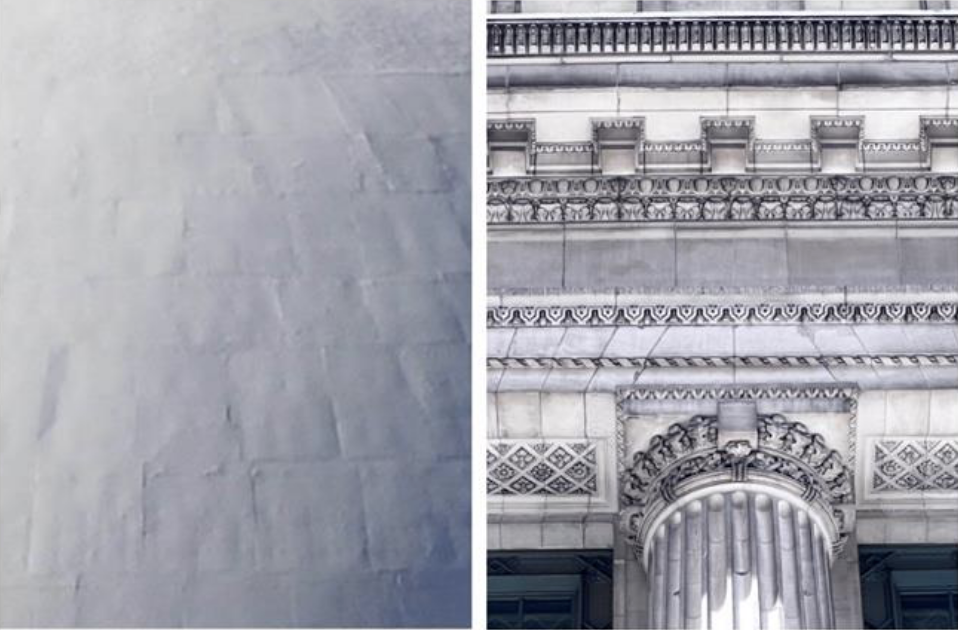
\includegraphics[height=4.75cm]{figures/beautyscale_image.png}
    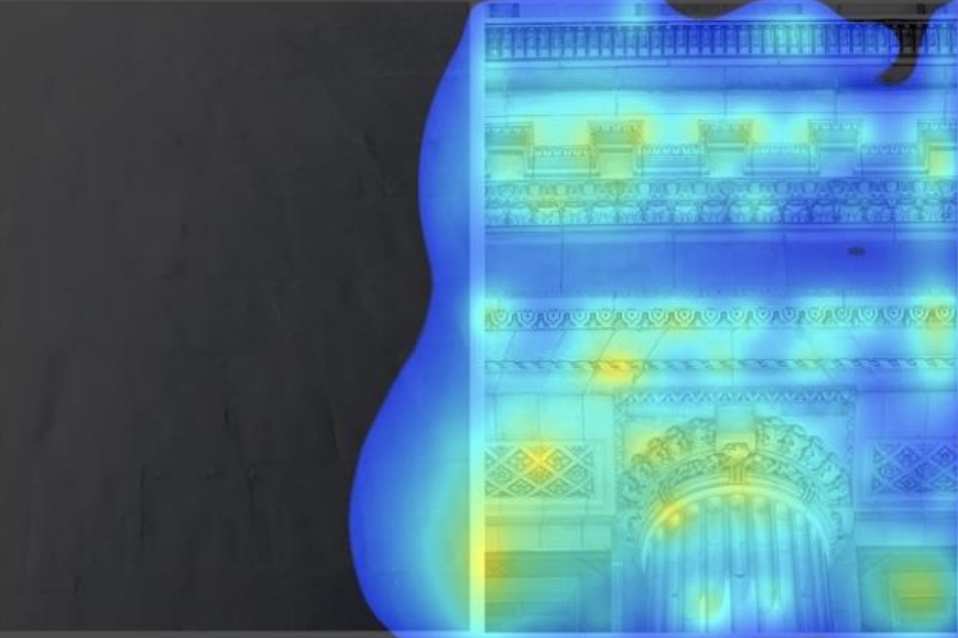
\includegraphics[height=4.75cm]{figures/beautyscale_heatmap.png}
    \captionof{figure}{Left: Two designs for a building facade. Right: A heatmap reveals the degree to which the two different facade designs capture the attention of study participants. The heatmap was generated from eye-tracking data. As expected, the feature-rich pillar capital and lower-side cornice of the right facade retains visual attention to a much higher degree. Source: Figure 6 from Lavdas' and Salingaros' seminal publication \textit{"Architectural Beauty: Developing a Measurable and Objective Scale"}}
    \label{fig:caricature_loos}
\end{mdframed}

\subsection{Architectural Beauty: Developing a Measurable and
Objective Scale}

(...) Lost among the heated and partisan media debate, a confluence of events occurred
that signals a paradigm shift. An independent Harris Poll revealed overwhelming pub-
lic preference for traditional versus modernist US federal buildings [13]. The pollsters
were able to show that this preference in no way depends upon political party affiliation.
Two separate groups of researchers verified the results of the Harris Poll with either direct
eye-tracking experiments, or eye-tracking simulation software [14,15]. Brandon Ro used vi-
sual attention software by 3M Corporation, while Ann Sussman measured eye movements
on webcams while subjects viewed the images on a computer screen. Evaluating the same
set of comparison image pairs from the Harris Poll, both research groups found complete
agreement with the survey results.

Several architectural organizations are trying to convince politicians to support bi-
ologically based objective beauty, and to block the wanton destruction of historical ur-
ban fabric that exemplifies those desirable qualities. One of these is Le Table Ronde de
l’Architecture in Belgium [16]. Co-author NAS is a signatory of their declaration. The
umbrella non-governmental organization The Architectural Uprising is active in the Baltic
and Scandinavian countries as well as in the United Kingdom [17], and its branches survey
the most beautiful versus ugliest new buildings in each country.

Psychologists have used numerical scales to measure beauty, starting with Gustav
Fechner in the 19th century [18]. We have hypothesized a method that could prove to be
useful if other researchers rigorously tested the methodology, and provide documentation
for the underlying assumptions and theories that drive the research hypothesis, design,
and execution, using established research protocols.

\subsection{Biologically Based Objective Beauty}

Medical practitioners are belatedly realizing that architectural culture’s dominant,
ingrained aesthetic is not compatible with laboratory measurements indicating salutogenic
environments [31–38]. The established approach to design undermines recent trends in
using the environment to significantly aid in healing. This effort includes, but is not limited
to, biophilic effects of human health. The healthcare profession does not know how the
curriculum for training architects omits any discussion of the opposing valence sets of
sensory qualities linked to beauty. Students are conditioned to disengage from neurological
responses occurring in their own bodies, which is the reason why they—as practicing
architects—later have such a psychological resistance to diagnosing objective beauty in the
designed environment [39].

Going beyond generic design minimalism that lacks biophilic healing properties, the
architecture profession imitates pathological conditions. Trauma survivors can lose their
ability to process complex visual detail: yet a visually empty and featureless building delib-
erately banishes ordered architectural detail. Depressingly grey minimalistic design styles
mimic pathologies of the eye-brain system such as cataract, Carbon Monoxide poisoning,
cerebral achromatopsia, cortical lesions, macular degeneration, retinal detachment, and
visual agnosia [40] (Chapter 4). This medically inexplicable choice generates anxiety in
users; however, it advocates a preferred and subjective architectural aesthetic.

Substantial evidence exists for the effect that stress, and stressful urban environments,
have on facial beauty [41]. A combination of stressors, mainly visual, affect the entire
body, altering facial features so that they are perceived as being “uglier” than normal (a
relative, not absolute measure), summarized as “stress induces ugliness”. However, also
the other way around: ugliness induces stress. Experiments to establish the dual effect
use medical evidence to measure stress, but the tools for measuring “ugliness” need an
objective method of measuring architectural beauty.
It turns out that ugliness in the visual environment induces facial stress in the observer,
which manifests in measurable though non-obvious facial features. AI-based programs discover the effect that environmental stress has by generating ugliness in a person’s
face, which reciprocates with ugliness in the built environment generating stress in the
human body.

Current technology makes possible computer-based facial expression recognition.
Among several companies offering diagnostic products for facial expression analysis,
iMotions and Noldus companies have established commercial platforms [42,43]. These
similar tools sense how detailed facial features respond to an image and use AI to infer
the unconscious emotional responses. The method “reads” facial muscle activity, which
evolution has specialized for expression. Affectiva company (owned by Smart Eye, which
also owns iMotions) is pioneering emotion AI software that measures human emotions
and complex cognitive states by supplementing facial movements with other biometric
sensors [44].
The capability of measuring environmental ugliness indirectly through physiological
sensors represents a paradigm shift for design. Physiological stress induced by specific
types of environmental information—which are identified as “ugly”—generates patholo-
gies. This normally unnoticed mechanism of interacting visually with the environment
goes beyond aesthetics, to influence human health. We expect forthcoming experiments to
unambiguously support quantitative methods of ranking architectural beauty. The existing
applications are to fine art, however, and not architecture.

\subsection{Why the Beauty Scale Generates Cognitive Dissonance in Architects}

Beauty does lie in the eye of the beholder, but this does not mean that it is arbitrarily
defined on a subjective basis [94]. Architects have trouble with the beauty scale as a
consequence of their training, and voice an opposite opinion from their built-in biological
instincts. Asking the beauty-scale question sparks cognitive dissonance since modernist
tradition teaches a predisposition that reverses unconscious responses. Architects are
taught a subjective set of aesthetics, and at the same time, they have to suppress their
innate sensory experience in favor of a learned preference. Fear—influenced by aesthetic
opinions based on group preference—sabotages the sensory basis for judging something
on the beauty scale.

Conditioned architects keep their neurological responses in check when identifying
dehumanizing grey concrete surfaces as “beautiful” [95]. They automatically rate a rough
Brutalist wall at 10, even though their own body tells them it’s depressing and repul-
sive, hence rating a 0. This tension produces cognitive dissonance [96]. At the high end
of the beauty scale, color, organized complexity, and ornament cause anxiety for PTSD
(Post-Traumatic Stress Disorder) and autistic subjects, who seek psychological relief in
minimalist environments. Ann Sussman suggests that signs of Autism Spectrum Disorder
(ASD) and PTSD after WWI in the pioneers of modernist architecture could help explain
diminished ability to process complex visual stimuli — including an aversion to face-like
symmetries [55,97,98]. Neurotypical architecture students are imbued with those pref-
erences, compelling them to score a building at 0 that actually ranks a 10 in biological
terms [39,40,96].

Architectural education uses operant conditioning to achieve the unnatural goal of
devaluing biological beauty. Confronted with “approved” styles with minimal values
of objective beauty, students are rewarded for propagating them, and become afraid of
their own innate ability to feel pleasure from sources of coherent complex information. As
Brielmann and Pelli [18] showed, an experience of beauty occurs when pleasure is high
and is unlikely to occur when little pleasure is felt. Therefore, suppressing pleasure is a
necessary prerequisite to suppressing biologically based beauty. The inability to experience
pleasure is called anhedonia. Architects are taught emotional cutoff: to be unreceptive to
visceral pleasure coming from the environment.

The neurological pathways that encode valences (i.e., bad versus good emotional
associations) are known. It is possible to reverse valences established through memory:
conditioning achieves a valence switch [99]. In Brave New World, Aldous Huxley describes
babies being conditioned to hate flowers and pretty images of animals, so as “to abolish
the love of nature” [100]. For the past century, architectural education has focused on
training exercises that achieve emotional numbing with respect to the environment, as a
means to switch valences [39]. Prior conditioning explains why design professionals show
insensitivity to the feelings of users inhabiting their work.

\clearpage
\section{Architecture and Democracy}

\begin{mdframed}[linewidth=1pt, roundcorner=5pt, innerleftmargin=10pt, innerrightmargin=10pt, innertopmargin=10pt, innerbottommargin=10pt, linecolor=black, backgroundcolor=white, userdefinedwidth=\textwidth]
    Switzerland is consistently ranked as one of the most democratic nations globally \cite{noauthor_economist_2023} with the principles of subsidiarity and direct democracy forming a vital part of Swiss national identity. Meanwhile, the ability of individuals to actively participate or shape the built environment, sometimes described as \textit{the art that we live in} \cite{hughes_shock_1980}, remains fundamentally limited. Home ownership in Switzerland remains elusive for the majority of the population, having stagnated at around 40\% over the past decades \cite{noauthor_home_2022}. At the same time, the majority of rental properties are built, owned and managed by large corporations or pension funds \cite{noauthor_wem_nodate}. These owners, in the ever supply-constrained real estate market, have little incentive to build aesthetically pleasing homes. And even in the case of representative (government) buildings, the public is rarely consulted in selecting the design. This means that aesthetic decisions are ultimately far removed from the primary aesthetic stakeholders: the general public. The \textit{Architecture Uprising}, an international movement originating in Sweden, has been successfully advocating for this to change. The below material provides an overview of this movement - and the advocacy of Michael Diamant, one of its leading figures.
\end{mdframed}

\subsection{The Aesthetic City YouTube Channel}

\noindent
\begin{minipage}[t]{0.49\linewidth}
    \centering
    
\includegraphics[width=\linewidth]{./figures/thumbnail_interview.jpg}
    \href{https://youtu.be/a9uLNxyKgCE?si=srT0AzgzI3LR4ccr}{Michael Diamant: The Origins of the Uprising}
\end{minipage}%
\hfill
\begin{minipage}[t]{0.49\linewidth}
    \centering
    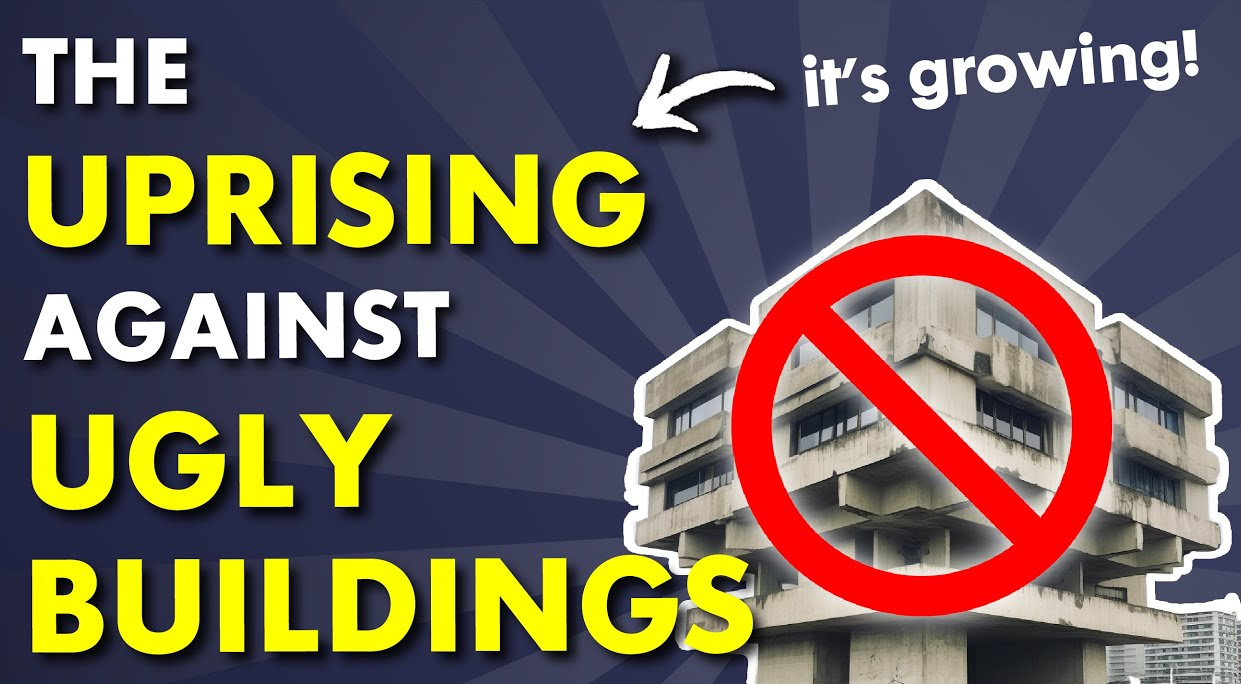
\includegraphics[width=\linewidth]{./figures/thumbnail_uprising.jpg}
    \href{https://youtu.be/NTGQ_kITzmY?si=yEBpKZUstUKUUOqp}{"The Revolution Changing Architecture"}
\end{minipage}

\subsection{Excerpts from a Bloomberg Article \cite{gersten_nordic_2023} on the \textit{Architecture Uprising}}

(...) Founded in Sweden in 2014 as a public Facebook group, the Uprising is a collective of citizen design critics who object to what organizers call the “continued uglification” of developments in Nordic cities, and push for a return to classically informed design. With more than 100,000 social media followers across some 40 different branches, the group now serves as a significant platform for those who assert that the public, not just bureaucrats, architects, developers and property owners, ought to have a voice in the design of their built environments. (...)

Passion (...) is the point. “There needs to be anger,” says Michael Diamant, a co-founder of the Swedish branch who works by day as a hospital personnel manager. \textit{“People have the right to be angry, because all the ugliness they see is on purpose, and if we speak out we’re called conservative. But yes, we can build beautiful and new. We have to create a lot of noise, otherwise nothing will change." }(...) Uprisings have since caught on in Germany, Estonia, Poland, the Netherlands and even the US. In Norway, with local parliamentary elections around the corner, Lie says, the group is realizing that there is indeed power in numbers. \textit{“We are being contacted by politicians who want to meet with us, have us on their podcasts, ask our opinions,”} Lie says.

Olsson, the Swedish Uprising moderator, easily recalls his favorite accomplishment as a member of the movement: the Gothenburg building Ekmansgatan 5, originally proposed as a modernist structure, that was re-envisioned in a classical style in the years after Olsson wrote up his objection to the design on the Swedish Uprising’s blog in 2018. \textit{“At first I was like, was this because of what I wrote, or was it a coincidence?”} Olsson recalled. \textit{“But I’ve heard from people that it was probably my text that changed it.”} The first time Olsson visited the building, when it was nearly finished, a stranger stopped beside him to admire the construction. \textit{“He said to me, ‘You know, this building is so beautiful. I don’t get why they don’t build like this all the time.’”}

\clearpage

\section{Architecture and Sustainability}



\clearpage

\printbibliography

\end{document}